\documentclass[tikz,border=7pt]{standalone}
\usepackage{pgfplots}
\pgfplotsset{compat=1.18}
\begin{document}
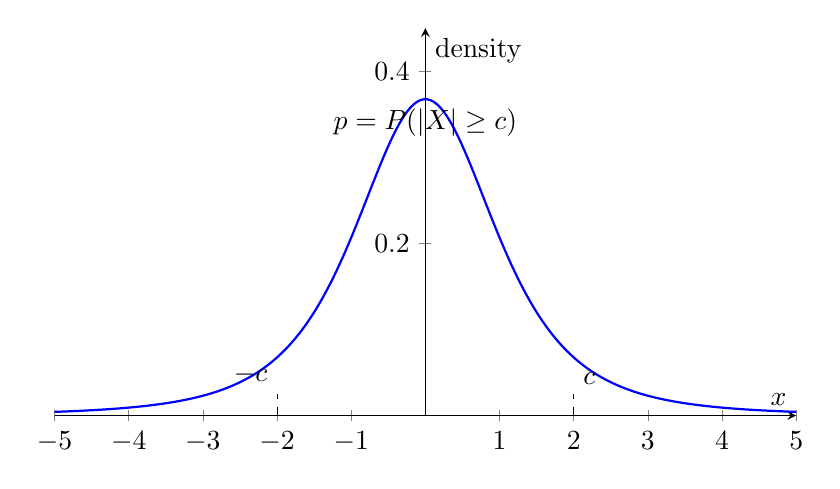
\begin{tikzpicture}
\begin{axis}[width=11cm,height=6.5cm,axis lines=middle,xmin=-5,xmax=5,ymin=0,ymax=.45,samples=220,xlabel={$x$},ylabel={density}]
\addplot[blue,thick,domain=-5:5] {.367553*(1+x^2/3)^(-2)};
\addplot[blue!25,draw=none,domain=-5:-2] {.367553*(1+x^2/3)^(-2)} \closedcycle;
\addplot[blue!25,draw=none,domain=2:5] {.367553*(1+x^2/3)^(-2)} \closedcycle;
\draw[dashed] (axis cs:-2,0)--(axis cs:-2,.025) node[above left] {$-c$};
\draw[dashed] (axis cs:2,0)--(axis cs:2,.025) node[above right] {$c$};
\node at (axis cs:0,.34) {$p=P(|X|\ge c)$};
\end{axis}
\end{tikzpicture}
\end{document}
